\documentclass[unnumsec,webpdf,modern,large]{projet_manifold}%

%\usepackage{showframe}
\usepackage{titlesec}
\usepackage{subcaption}
% Définition des styles pour les différents niveaux de titres
\titleformat{\section}
  {\normalfont\Large\bfseries}{\thesection}{1em}{}
\titleformat{\subsection}
  {\normalfont\large\bfseries}{\thesubsection}{1em}{}
\titleformat{\subsubsection}
  {\normalfont\normalsize\bfseries}{\thesubsubsection}{1em}{}
\titleformat{\paragraph}
  {\normalfont\normalsize\bfseries}{\theparagraph}{1em}{}

% Activation de la numérotation pour les paragraphes
\setcounter{secnumdepth}{4}

\graphicspath{{Fig/}}
\usepackage{hyperref}
% line numbers
%\usepackage[mathlines, switch]{lineno}
%\usepackage[right]{lineno}

\theoremstyle{thmstyleone}%
\newtheorem{theorem}{Theorem}%  meant for continuous numbers
%%\newtheorem{theorem}{Theorem}[section]% meant for sectionwise numbers
%% optional argument [theorem] produces theorem numbering sequence instead of independent numbers for Proposition
\newtheorem{proposition}[theorem]{Proposition}%
%%\newtheorem{proposition}{Proposition}% to get separate numbers for theorem and proposition etc.
\theoremstyle{thmstyletwo}%
\newtheorem{example}{Example}%
\newtheorem{remark}{Remark}%
\theoremstyle{thmstylethree}%
\newtheorem{definition}{Definition}


\begin{document}
\journaltitle{Travail de Synthèse Cours Manifold Learning, semestre 1 MALIA}
\DOI{ objet numérique sans identifiant (préparation pédagogique) }
\copyrightyear{2024}
\pubyear{2024}
\access{Date de soumission : octobre 2024}
\appnotes{Supervisé par : Dr Jairo Cugliari Duhalde}

\firstpage{1}

%\subtitle{Subject Section}

\title[Short Article Title]{Étude Comparative Des Algorithmes : PCA, ISOMAP, LLE et Auto-Encoders }


\author[1,$\ast$]{Mehdi Mansour}


\authormark{M.Mansour et al.}

\address[1]{\orgdiv{Departement Informatique}, \orgname{ICOM}, \orgaddress{\street{5 avenue Pierre Mendès France}, \postcode{69500 Bron},  \country{France}}}


\corresp[*]{Corresponding author. \href{mailto:mehdi.mansour@univ-lyon2.fr}{mehdi.mansour@univ-lyon2.fr}}

%\received{Date}{0}{Year}
%\revised{Date}{0}{Year}
%\accepted{Date}{0}{Year}

\abstract{
Cette étude comparative examine les performances de quatre algorithmes de réduction de dimensionnalité: l'Analyse en Composantes Principales (PCA), ISOMAP, l'Apprentissage de Variétés Localement Linéaires (LLE), et les Auto-Encoders. Nous avons évalué ces algorithmes sur des ensembles de données synthétiques (disque, hélice, Swiss roll ondulé) ainsi que sur le jeu de données réel Fashion-MNIST. Notre analyse se concentre sur la capacité de ces méthodes à préserver la structure et l'information des données dans un espace de dimension réduite. Les résultats obtenus corroborent les conclusions de l'état de l'art, démontrant les forces et les limites de chaque approche selon la nature des données traitées. Cette étude, réalisée dans un cadre scolaire, offre un aperçu pratique des différentes techniques de manifold learning et de leur applicabilité dans divers contextes.
}

\keywords{Réduction de dimensionnalité, PCA, ISOMAP, LLE, Auto-Encoders, Manifold Learning, Fashion-MNIST}

% \boxedtext{
% \begin{itemize}
% \item Key boxed text here.
% \item Key boxed text here.
% \item Key boxed text here.
% \end{itemize}}


\maketitle

%%%%%%%%%%%%%%%%%%%%%%%%%%%%%%%%%%%%%%%%%%%%%%%%%%%%%%%%%%%%%%%%%%%%%%%%%%%%%%%%%%%%%%%%%%%%%%%%%%%%%%%%%%%%%%%%%%%%%%%%%%%%%%%%%%%%%%%%%%%%%%%%%%%%%%%%%%%%%%%%%%%%%%%%

\section{Introduction}
La réduction de dimensionnalité est une technique fondamentale en apprentissage automatique et en analyse de données, visant à représenter des données de haute dimension dans un espace de dimension inférieure tout en préservant les caractéristiques essentielles. Cette approche est cruciale pour surmonter le "fléau de la dimensionnalité", améliorer l'efficacité computationnelle, et faciliter la visualisation et l'interprétation des données \cite{vandermaaten2009dimensionality}.

Dans cette étude, nous nous concentrons sur quatre méthodes de réduction de dimensionnalité largement utilisées : l'Analyse en Composantes Principales (PCA), ISOMAP, l'Apprentissage de Variétés Localement Linéaires (LLE), et les Auto-Encoders. Chacune de ces méthodes présente des caractéristiques uniques :

\begin{itemize}
    \item La PCA est une technique linéaire qui projette les données sur les axes de variance maximale \cite{jolliffe2002principal}.
    \item ISOMAP cherche à préserver les distances géodésiques entre les points dans un espace de dimension réduite \cite{tenenbaum2000global}.
    \item LLE tente de reconstruire chaque point comme une combinaison linéaire de ses voisins \cite{roweis2000nonlinear}.
    \item Les Auto-Encoders utilisent des réseaux de neurones pour apprendre une représentation compressée des données \cite{hinton2006reducing}.
\end{itemize}

Notre objectif est de comparer ces méthodes sur des ensembles de données synthétiques, en évaluant leur capacité à préserver la structure des données et à capturer des relations non linéaires. Cette comparaison vise à fournir des insights sur les forces et les faiblesses de chaque méthode dans différents contextes. Une méthode parmis les quatre sera candidate à effectuer ce travail sur un dataset conséquent du réel, afin de vérifier la robustesse des conclusions lors d'une application sur des données volumineuses et potentiellement bruitées.

%%%%%%%%%%%%%%%%%%%%%%%%%%%%%%%%%%%%%%%%%%%%%%%%%%%%%%%%%%%%%%%%%%%%%%%%%%%%%%%%%%%%%%%%%%%%%%%%%%%%%%%%%%%%%%%%%%%%%%%%%%%%%%%%%%%%%%%%%%%%%%%%%%%%%%%%%%%%%%%%%%%%%%%

\section{Matériels et Méthodes}

%%%%%%%%%%%%%%%%%%%%%%%%%%%%%%%%%%%%%%%%%%%%%%%%%%%%%%%%%%%%%%%%%%%%%%%%%%%%%%%%%%%%%%%%%%%%%%%%%%%%%%%%%%%%%%%%%%%%%%%%%%%%%%%%%%%%%%%%%%%%%%%%%%%%%%%%%%%%%%%%%%%%%%%%

\subsection{Ensembles de Données}

Notre étude utilise cinq ensembles de données synthétiques soigneusement choisis pour représenter diverses structures de manifolds, ainsi qu'un ensemble de données réelles. Chaque ensemble synthétique a été généré avec et sans bruit gaussien (écart-type $\sigma = 0.05$) pour évaluer la robustesse des méthodes de réduction de dimensionnalité.

\subsubsection{Ensembles de Données Synthétiques}

\paragraph{Hélice Simple} 
Un manifold 1D enroulé dans un espace 3D, représenté par les équations paramétriques :
\begin{equation}
    x = \cos(t), \quad y = \sin(t), \quad z = t / (2\pi)
\end{equation}
où $t \in [0, 4\pi]$. Cette structure permet d'évaluer la capacité des algorithmes à "dérouler" un manifold non linéaire simple.

\paragraph{Double Hélice} 
Deux manifolds 1D enroulés, simulant une structure d'ADN, définis par :
\begin{align}
    x_1 &= r \cos(t), \quad y_1 = r \sin(t), \quad z_1 = t / (2\pi) \\
    x_2 &= r \cos(t + \pi), \quad y_2 = r \sin(t + \pi), \quad z_2 = t / (2\pi)
\end{align}
où $t \in [0, 4\pi]$ et $r = 1$. Ce dataset teste la capacité à distinguer et à préserver deux structures entrelacées.

\paragraph{Swiss Roll Ondulé} 
Un manifold 2D avec une petite ondulation sinusoïdale le long de sa surface, défini par :
\begin{equation}
    x = t \cos(t), \quad y = 21 \cdot \text{rand}(0,1), \quad z = t \sin(t) + A \sin(f \cdot y)
\end{equation}
où $t \in [1.5\pi, 4.5\pi]$, $A = 1$ (amplitude de l'ondulation) et $f = 1$ (fréquence). Cette structure complexe évalue la capacité à "déplier" un manifold non linéaire tout en préservant les relations locales.

\paragraph{Paraboloïde Hyperbolique} 
Un manifold 2D complexe en forme de selle, représenté par :
\begin{equation}
    z = \frac{x^2}{a^2} - \frac{y^2}{b^2}
\end{equation}
où $x, y \in [-2, 2]$ et $a = b = 1$. Cette surface quadrique teste la préservation des courbures positives et négatives dans un espace réduit.

\paragraph{Disque Incliné} 
Un manifold 2D plat mais incliné dans un espace 3D, défini par :
\begin{equation}
    x = r \cos(\theta), \quad y = r \sin(\theta) \cos(\phi), \quad z = r \sin(\theta) \sin(\phi)
\end{equation}
où $r \in [0, 1]$, $\theta \in [0, 2\pi]$, et $\phi = 60^\circ$ (angle d'inclinaison). Ce dataset évalue la capacité à reconnaître et à préserver une structure plane dans un espace 3D.

\begin{figure*}[t]
    \centering
    \begin{minipage}{0.19\textwidth}
        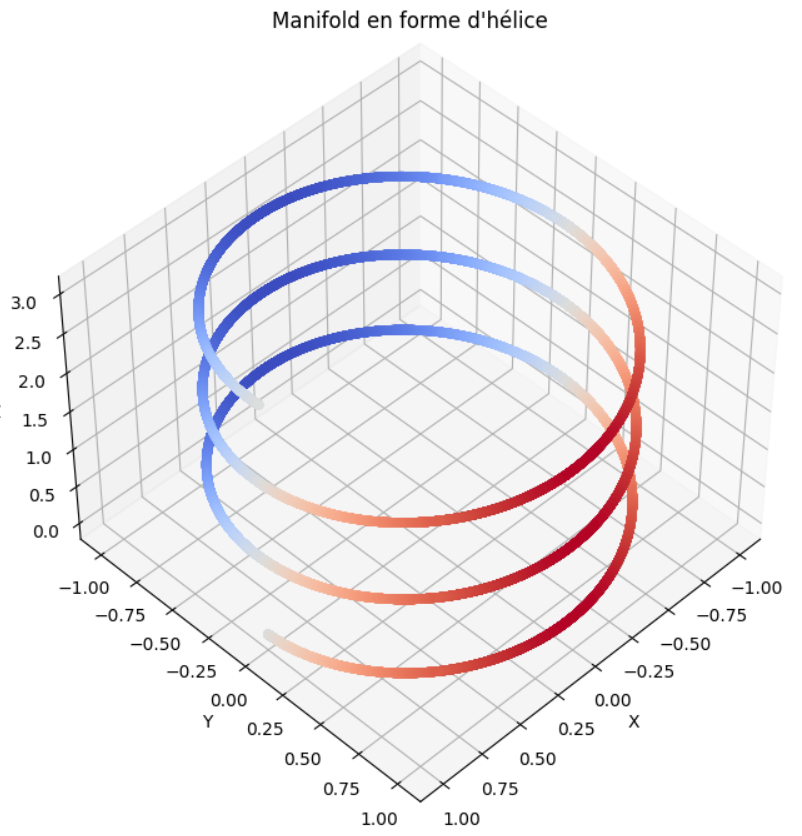
\includegraphics[width=\linewidth]{Fig/helice.png}
        \caption*{(a) Hélice}
    \end{minipage}%
    \hfill
    \begin{minipage}{0.19\textwidth}
        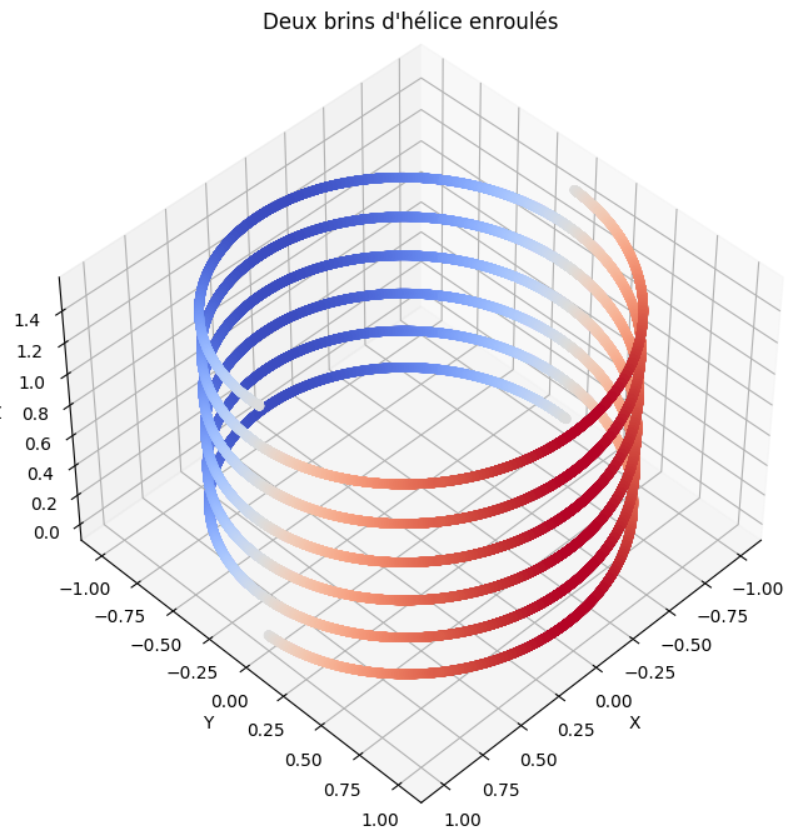
\includegraphics[width=\linewidth]{Fig/adn.png}
        \caption*{(b) ADN }
    \end{minipage}%
    \hfill
    \begin{minipage}{0.19\textwidth}
        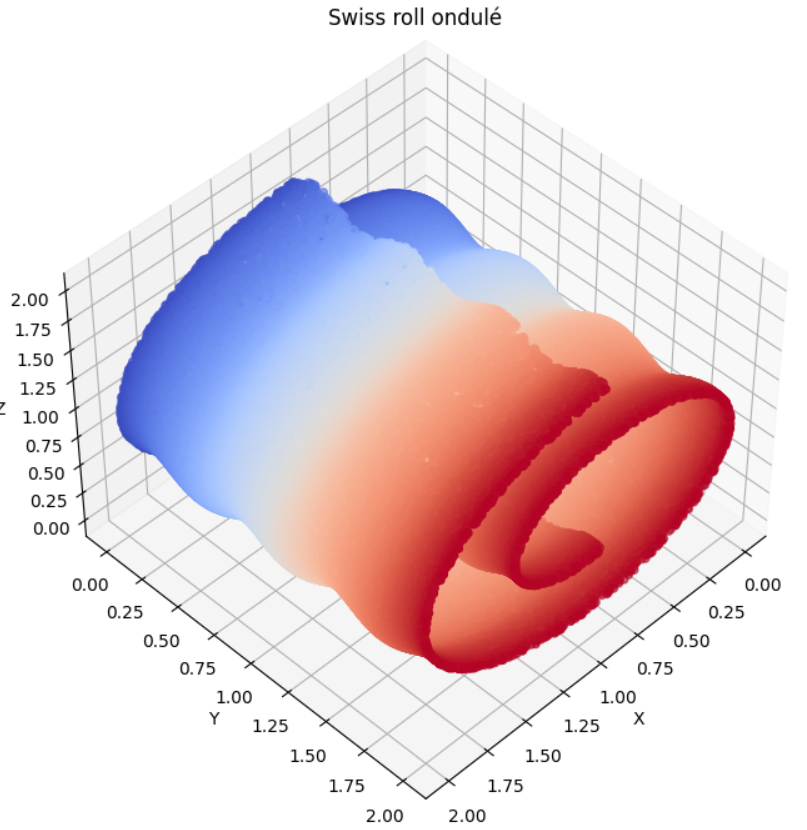
\includegraphics[width=\linewidth]{Fig/swiss_roll_ondule.png}
        \caption*{(c) Swiss Roll}
    \end{minipage}%
    \hfill
    \begin{minipage}{0.19\textwidth}
        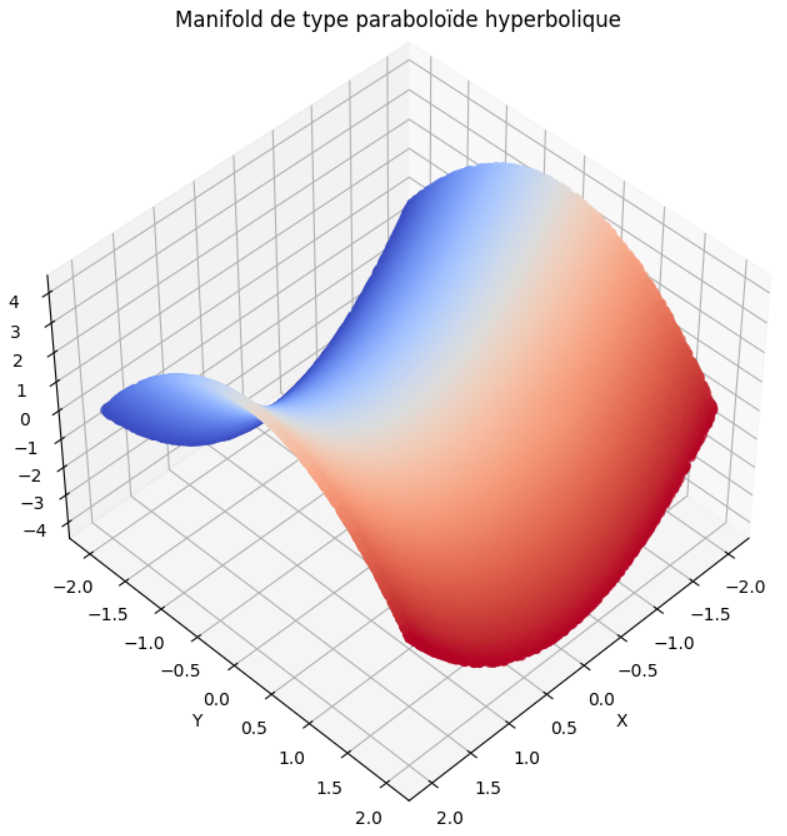
\includegraphics[width=\linewidth]{Fig/selle.png}
        \caption*{(d) Selle}
    \end{minipage}%
    \hfill
    \begin{minipage}{0.19\textwidth}
        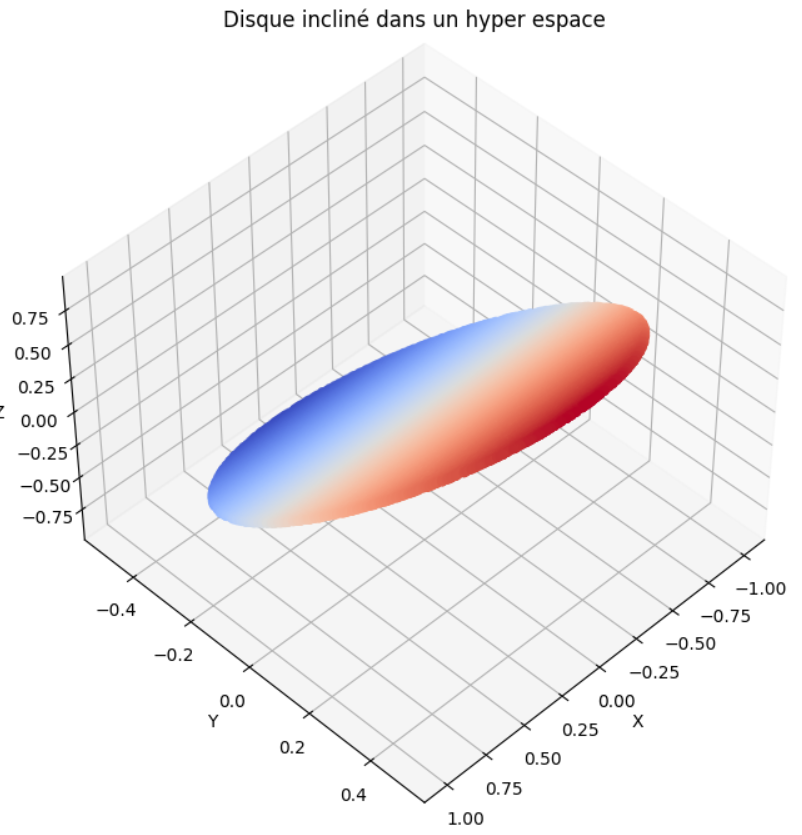
\includegraphics[width=\linewidth]{Fig/disque.png}
        \caption*{(e) Disque Incliné}
    \end{minipage}
    \caption{ Visualisation des ensembles de données synthétiques (ensemble des figures ci-dessus}
    \label{fig:synthetic_datasets}
\end{figure*}


%%%%%%%%%%%%%%%%%%%%%%%%%%%%%%%%%%%%%%%%%%%%%%%%%%%%%%%%%%%%%%%%%%%%%%%%%%%%%%%%%%%%%%%%%%%%%%%%%%%%%%%%%%%%%%%%%%%%%%%%%%%%%%%%%%%%%%%%%%%%%%%%%%%%%%%%%%%%%%%%%%%%%%%%


\subsubsection{Ensemble de Données Réelles : Fashion-MNIST}
Fashion-MNIST \cite{xiao2017fashion} est un ensemble de données de référence composé de 70 000 images en niveaux de gris de 28x28 pixels, représentant 10 catégories de vêtements et d'accessoires. Cet ensemble comprend 60 000 images d'entraînement et 10 000 images de test.
Les caractéristiques de Fashion-MNIST sont :
\begin{itemize}
    \item 10 classes : T-shirt/top, pantalon, pull-over, robe, manteau, sandale, chemise, basket, sac, bottine.
    \item Chaque image est représentée par un vecteur de 784 dimensions (28x28 pixels).
    \item Les valeurs des pixels sont normalisées entre 0 et 1.
\end{itemize}
La Figure \ref{fig:fashion_mnist_samples} présente des exemples d'images de chaque classe de Fashion-MNIST.

\begin{figure}[h]
    \centering
    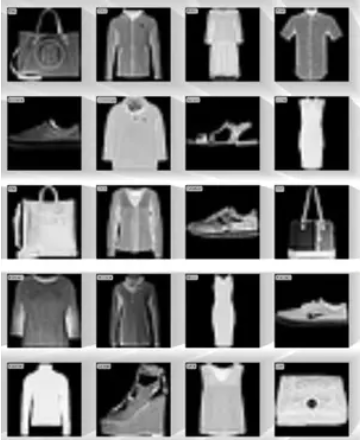
\includegraphics[width=\columnwidth]{Fig/fashion_mnist.png}
    \caption{Échantillons d'images de l'ensemble de données Fashion-MNIST, illustrant les 10 classes différentes.}
    \label{fig:fashion_mnist_samples}
\end{figure}

L'utilisation de Fashion-MNIST permet d'évaluer les performances des méthodes de réduction de dimensionnalité sur des données réelles de haute dimension, tout en offrant un contexte d'application concret dans le domaine de la vision par ordinateur et de la classification d'images.

La diversité de ces ensembles de données, allant de structures géométriques simples à des manifolds complexes et des données réelles, offre un cadre complet pour évaluer les forces et les faiblesses de chaque méthode de réduction de dimensionnalité étudiée.



%%%%%%%%%%%%%%%%%%%%%%%%%%%%%%%%%%%%%%%%%%%%%%%%%%%%%%%%%%%%%%%%%%%%%%%%%%%%%%%%%%%%%%%%%%%%%%%%%%%%%%%%%%%%%%%%%%%%%%%%%%%%%%%%%%%%%%%%%%%%%%%%%%%%%%%%%%%%%%%%%%%%%%%%
\subsection{Algorithmes utilisés}

Dans cette étude, nous avons implémenté et comparé quatre méthodes de réduction de dimensionnalité, chacune ayant ses propres fondements mathématiques et promesses théoriques :

\subsubsection{Analyse en Composantes Principales (PCA)}

\paragraph{Fondements mathématiques :}
La PCA est une technique linéaire qui projette les données sur les axes de variance maximale. Mathématiquement, pour un ensemble de données $X$ de dimension $n \times p$, la PCA cherche à trouver une matrice de projection $W$ telle que :

\begin{equation}
    Y = XW
\end{equation}

où $Y$ est la représentation réduite des données. $W$ est obtenue en résolvant le problème aux valeurs propres :

\begin{equation}
    C_X W = W \Lambda
\end{equation}

où $C_X$ est la matrice de covariance de $X$ et $\Lambda$ est une matrice diagonale des valeurs propres.

\paragraph{Promesses théoriques :}
\begin{itemize}
    \item Préservation optimale de la variance globale des données.
    \item Décorrélation des caractéristiques dans l'espace réduit.
    \item Garantie de reconstruction optimale au sens des moindres carrés.
\end{itemize}

\subsubsection{ISOMAP}

\paragraph{Fondements mathématiques :}
ISOMAP étend l'idée du Multi-Dimensional Scaling (MDS) en remplaçant les distances euclidiennes par des distances géodésiques estimées. Le processus se déroule en trois étapes :

1) Construction d'un graphe des k plus proches voisins.
2) Calcul des distances géodésiques entre tous les points en utilisant l'algorithme de Dijkstra.
3) Application du MDS classique sur la matrice des distances géodésiques.

La fonction objectif à minimiser est :

\begin{equation}
    E = \sum_{i<j} (d_G(x_i, x_j) - \|y_i - y_j\|)^2
\end{equation}

où $d_G$ est la distance géodésique et $y_i$, $y_j$ sont les coordonnées dans l'espace réduit.

\paragraph{Promesses théoriques :}
\begin{itemize}
    \item Préservation de la structure globale non linéaire des données.
    \item Convergence asymptotique vers la vraie structure du manifold sous certaines conditions.
    
\end{itemize}

\subsubsection{Locally Linear Embedding (LLE)}

\paragraph{Fondements mathématiques :}
LLE reconstruit chaque point comme une combinaison linéaire de ses voisins. Le processus comprend deux étapes principales :

1) Calcul des poids de reconstruction $W_{ij}$ en minimisant :

\begin{equation}
    \epsilon(W) = \sum_i \|x_i - \sum_j W_{ij}x_j\|^2
\end{equation}

2) Calcul des coordonnées de basse dimension $Y$ en minimisant :

\begin{equation}
    \Phi(Y) = \sum_i \|y_i - \sum_j W_{ij}y_j\|^2
\end{equation}

sous contraintes de centrage et d'échelle.

\paragraph{Promesses théoriques :}
\begin{itemize}
    \item Préservation des relations locales entre les points.
    \item Invariance aux rotations, translations et mises à l'échelle.
   
\end{itemize}

\subsubsection{Auto-Encodeurs}

\paragraph{Fondements mathématiques :}
Les auto-encodeurs sont des réseaux de neurones qui apprennent une représentation compressée (encodage) des données d'entrée, puis tentent de reconstruire ces données (décodage). Formellement, pour une entrée $x$, l'auto-encodeur apprend une fonction d'encodage $f$ et une fonction de décodage $g$ telles que :

\begin{equation}
    \hat{x} = g(f(x))
\end{equation}

où $\hat{x}$ est la reconstruction de $x$. L'objectif est de minimiser l'erreur de reconstruction :

\begin{equation}
    L(x, \hat{x}) = \|x - \hat{x}\|^2
\end{equation}

\paragraph{Promesses théoriques :}
\begin{itemize}
    \item Capacité à capturer des relations hautement non linéaires.
    \item Flexibilité dans la conception de l'architecture pour s'adapter à différents types de données.
    \item Possibilité d'intégrer des contraintes spécifiques au domaine dans le processus d'apprentissage.
\end{itemize}

Chacune de ces méthodes offre une approche unique pour aborder le problème de la réduction de dimensionnalité, avec des forces et des limitations spécifiques que nous explorerons à travers nos expériences sur les datasets synthétiques et réels.


%%%%%%%%%%%%%%%%%%%%%%%%%%%%%%%%%%%%%%%%%%%%%%%%%%%%%%%%%%%%%%%%%%%%%%%%%%%%%%%%%%%%%%%%%%%%%%%%%%%%%%%%%%%%%%%%%%%%%%%%%%%%%%%%%%%%%%%%%%%%%%%%%%%%%%%%%%%%%%%%%%%%%%%%
\section{Protocole Expérimental}

Notre étude comparative a suivi un protocole expérimental  conçu pour évaluer équitablement les performances de chaque méthode de réduction de dimensionnalité sur différents ensembles de données, Voici les détails de notre approche :

\subsection{Préparation des Données}

\subsubsection{Ensembles de Données Synthétiques}
Pour la génération des datasets synthétiques, nous avons procédé comme suit :

\begin{itemize}
    \item Génération des coordonnées 3D initiales selon les équations spécifiques à chaque manifold.
    \item Enrichissement de 97 dimensions supplémentaires avec des coordonnées tirées aléatoirement d'une distribution normale, puis normalisées pour garder une variance acceptable qui ne phagocyte pas la variance du vrai manifold.
    \item Création de deux versions de chaque dataset : une sans bruit et une avec un bruit gaussien (écart-type $\sigma = 0.05$) ajouté aux 100 dimensions.
\end{itemize}

Cette approche nous a permis de simuler des données de haute dimension tout en préservant la structure sous-jacente du manifold original.

\subsubsection{Ensemble de Données Réelles : Fashion-MNIST}

Pour notre étude sur des données réelles, nous avons utilisé le dataset Fashion-MNIST \cite{xiao2017fashion} avec des auto encodeurs convolutifs. Ce choix offre un bon compromis entre complexité et taille de données:

\begin{itemize}

    \item \textbf{Prétraitement} :
    \begin{itemize}
        \item Normalisation : Les valeurs des pixels ont été normalisées entre 0 et 1 en divisant par 255.
        \item Reshape : Les images ont été redimensionnées de (28, 28) à (28, 28, 1) pour être compatibles avec l'architecture d'entrée des auto encodeurs convolutifs.
    \end{itemize}
\end{itemize}

\subsection{Infrastructure de Calcul}

Les expérimentations ont souvent dû être répétées et certains calculs étaient conséquents. Le risque était de bloquer l'avancement du travail ou de limiter le champ des explorations à des valeurs très réduites et optimisées de manière caricaturale. Pour contourner cet inconvénient, le choix a été de s'appuyer autant que possible sur des infrastructures matérielles et des algorithmes permettant d'accélérer les calculs :

\begin{itemize}
    \item \textbf{GPU NVIDIA A100} : Accélération matérielle pour les opérations de calcul matriciel et l'entraînement des réseaux de neurones.
    
    \item \textbf{Librairies du projet "RAPIDS.ai"} : Implémentation GPU-accélérée des algorithmes standards de machine learning et de calcul matriciel, telles que cuML comme substitut rapide de scikit-learn ou cupy en alternative à numpy.
    
    \item \textbf{TensorFlow avec support GPU} : Utilisé pour l'implémentation et l'entraînement des auto encodeurs.
    
    \item \textbf{Alternatives sur CPUs multicœurs} : Certains algorithmes n'avaient pas d'implémentation compatible avec l'accélération sur GPU, comme ISOMAP. Nous avons utilisé un maximum de cœurs de CPU en définissant le paramètre \texttt{n\_jobs=-1} dans les méthodes qui le permettaient.
\end{itemize}


\subsection{Optimisation des Hyperparamètres}

Dans le cadre de notre étude comparative des méthodes de réduction de dimensionnalité, le calibrage des hyperparamètres est une étape cruciale pour garantir des performances optimales de chaque algorithme. Traditionnellement, des techniques telles que la validation croisée avec recherche sur grille (\textit{Grid Search}) ou aléatoire (\textit{Random Search}) sont utilisées. Cependant, ces approches peuvent être inefficaces en termes de temps de calcul et ne sont pas adaptées aux espaces de recherche de grande dimension ou complexes.

Pour surmonter ces limitations, nous avons opté pour l'utilisation d'Optuna \cite{akiba2019optuna}, un framework d'optimisation d'hyper-paramètres automatisé et efficace. Optuna permet une exploration intelligente de l'espace des hyperparamètres en utilisant des techniques d'optimisation bayésienne, notamment l'algorithme TPE (\textit{Tree-structured Parzen Estimator}).

\subsubsection{Pourquoi Optuna ?}

Optuna offre plusieurs avantages qui le rendent particulièrement adapté à notre étude :

\begin{itemize} \item \textbf{Optimisation efficace} : Utilise des méthodes d'optimisation séquentielle basée sur des modèles (SMBO), ce qui permet d'explorer l'espace des hyperparamètres de manière plus efficace que les recherches exhaustives. \item \textbf{Flexibilité} : Permet de définir des espaces de recherche complexes, incluant des hyperparamètres discrets, continus et catégoriels. \item \textbf{Pruning adaptatif} : Peut interrompre précocement les essais non prometteurs, économisant ainsi des ressources computationnelles. \item \textbf{Intégration facile} : S'intègre aisément avec les frameworks de machine learning courants tels que Scikit-learn et TensorFlow. \end{itemize}

\subsubsection{Fondements Mathématiques d'Optuna}

L'algorithme principal utilisé par Optuna pour l'optimisation des hyperparamètres est le TPE (\textit{Tree-structured Parzen Estimator}). Le TPE est une méthode d'optimisation bayésienne qui modélise la fonction objectif en utilisant des estimations de densité de probabilité.

\paragraph{Principe du TPE}

Le TPE cherche à modéliser la probabilité inverse $p(x|y)$ plutôt que la probabilité directe $p(y|x)$. Pour ce faire, il divise les observations en deux groupes :

\begin{itemize} \item $l(x)$ : Distribution des hyperparamètres ayant conduit à des performances "bonnes", c'est-à-dire avec une valeur de la fonction objectif inférieure à un seuil $y^\ast$. \item $g(x)$ : Distribution des hyperparamètres ayant conduit à des performances "mauvaises", c'est-à-dire avec une valeur de la fonction objectif supérieure ou égale à $y^\ast$. \end{itemize}

L'objectif est de choisir les hyperparamètres $x$ qui maximisent le rapport d'acquisition :

\begin{equation} \mathrm{EI}(x) = \frac{l(x)}{g(x)} \end{equation}

où $\mathrm{EI}(x)$ est l'\textit{Expected Improvement} (amélioration espérée).

\paragraph{Processus d'Optimisation}

Le processus se déroule en plusieurs étapes :

\begin{enumerate} \item \textbf{Définition de l'espace de recherche} : L'utilisateur spécifie les hyperparamètres à optimiser et leurs domaines respectifs. \item \textbf{Échantillonnage} : Optuna propose un ensemble d'hyperparamètres en maximisant le rapport $\frac{l(x)}{g(x)}$. \item \textbf{Évaluation} : Le modèle est entraîné avec ces hyperparamètres et la performance est évaluée. \item \textbf{Mise à jour des distributions} : Les distributions $l(x)$ et $g(x)$ sont mises à jour avec les nouvelles observations. \item \textbf{Itération} : Le processus est répété jusqu'à atteindre un critère d'arrêt (nombre maximal d'essais, convergence, etc.). \end{enumerate}

\paragraph{Pruning Adaptatif}

Optuna intègre également des techniques de \textit{pruning} adaptatif, basées sur des algorithmes tels que Successive Halving et Hyperband. Le principe est d'arrêter précocement les essais dont les performances intermédiaires sont inférieures à celles attendues, permettant ainsi de concentrer les ressources sur les configurations prometteuses.

\subsubsection{Application à nos Méthodes}

Pour chaque algorithme de réduction de dimensionnalité, nous avons défini un espace de recherche spécifique :

\begin{itemize} 
    \item \textbf{PCA} : Optimisation du nombre de composantes principales $n_{\text{components}} \in [2, 10]$. 
    \item \textbf{ISOMAP} : Optimisation du nombre de voisins $n_{\text{neighbors}} \in [4, 30]$ et du nombre de composantes $n_{\text{components}} \in [2, 10]$. 
    \item \textbf{LLE} : Optimisation du nombre de voisins $n_{\text{neighbors}} \in [5, 30]$ et du nombre de composantes $n_{\text{components}} \in [2, 10]$. 
    \item \textbf{Auto-Encodeurs} : Optimisation du nombre de couches $n_{\text{layers}} \in [2, 5]$, du nombre de neurones par couche $n_{\text{neurons}} \in \{64, 128, 256\}$, du taux de drop-out $\text{dropout\_rate} \in [0.0, 0.5]$ et de la taille de la couche latente $n_{\text{components}} \in [2, 10]$. 
\end{itemize}



Aussi, La fonction objectif à minimiser ou maximiser a été adaptée à chaque méthode :

\begin{itemize} \item \textbf{PCA} : Maximisation de la variance expliquée cumulée par les composantes retenues. \item \textbf{ISOMAP et LLE} : Minimisation de l'erreur de reconstruction géodésique ou locale. \item \textbf{Auto-Encodeurs} : Minimisation de l'erreur de reconstruction (MSE) entre les données originales et reconstruites. \end{itemize}

\subsubsection{Critères d'Arrêt et Paramètres d'Optimisation}

Nous avons fixé un nombre maximal d'essais (50 essais par étude) pour l'optimisation, en veillant à trouver un équilibre entre le temps de calcul et la qualité de l'optimisation. Le \textit{pruning} adaptatif d'Optuna a permis de réduire le temps de calcul en arrêtant précocement les configurations non prometteuses.

\subsection{Procédure d'Évaluation}

Pour évaluer les performances de chaque méthode de réduction de dimensionnalité avec les hyperparamètres optimisés, nous avons suivi une procédure en plusieurs étapes :

\subsubsection{Récupération des coordonnées dans l'espace réduit}

Chaque méthode a été appliquée sur les ensembles de données synthétiques et réels en utilisant les meilleurs hyperparamètres trouvés par Optuna. Cela garantit que chaque algorithme est évalué dans ses conditions optimales.

\subsubsection{Évaluation Quantitative}

Nous avons mesuré plusieurs métriques pour quantifier les performances :

\begin{itemize} 
    \item \textbf{Erreurs de Reconstruction} : Dans le cas d'Isomap par exemple, l'erreur de reconstruction est calculée en comparant la matrice des distances géodésiques centrées dans l'espace original et les valeurs propres obtenues dans l'espace réduit. La formule utilisée est :
    \begin{equation}
    E = \frac{\sqrt{\sum (G_{\text{center}}^2) - \sum (\lambda^2)}}{n}
    \end{equation}
    où $G_{\text{center}}$ est la matrice des distances géodésiques centrée dans l'espace d'origine, et $\lambda$ sont les valeurs propres résultantes de la décomposition KernelPCA dans l'espace réduit. Cette erreur quantifie dans quelle mesure l'embedding réduit capture la structure géométrique des distances dans l'espace d'origine.


    \item \textbf{Préservation des Distances Globales} : Évaluée à l'aide de la mesure de stress géodésique, qui quantifie la distorsion des distances globales lors de la réduction de dimensionnalité. Cette mesure est particulièrement adaptée pour des méthodes comme **Isomap**, qui cherchent à préserver les distances géodésiques sur le manifold. Le stress est calculé comme suit :
    \begin{equation}
    S_{\text{Isomap}} = \sqrt{\frac{\sum_{i < j} (d_{ij}^{\text{geo}} - d_{ij}^{\text{low}})^2}{\sum_{i < j} (d_{ij}^{\text{geo}})^2}}
    \end{equation}
    où $d_{ij}^{\text{geo}}$ est la distance géodésique dans l'espace de haute dimension, et $d_{ij}^{\text{low}}$ est la distance dans l'espace réduit. Un stress faible indique une bonne préservation des distances géodésiques globales et de la structure globale du manifold.

\item \textbf{Préservation des Distances Locales} : Évaluée à l'aide d'une mesure de stress local, qui quantifie la distorsion des distances entre un point et ses voisins immédiats. Cette mesure est adaptée pour des méthodes comme **LLE**, qui visent à préserver les relations locales entre les points. Le stress local est calculé comme suit :
    \begin{equation}
    S_{\text{LLE}} = \sqrt{\frac{\sum_{i < j, j \in N(i)} (d_{ij}^{\text{high}} - d_{ij}^{\text{low}})^2}{\sum_{i < j, j \in N(i)} (d_{ij}^{\text{high}})^2}}
    \end{equation}
    où $d_{ij}^{\text{high}}$ est la distance dans l'espace de haute dimension, et $d_{ij}^{\text{low}}$ est la distance dans l'espace réduit pour les points $j$ dans le voisinage immédiat $N(i)$ de $i$. Un stress faible indique une bonne préservation des relations locales entre les points voisins.

    \item \textbf{Performance de Classification} : Pour l'ensemble de données Fashion-MNIST, nous avons entraîné un classifieur de type regréssion logistique multinomiale sur les données en espace réduit et non-réduit et comparé l'exactitude des prédiction.
\end{itemize}


\subsubsection{Évaluation Qualitative}

Nous avons également réalisé une analyse visuelle :

\begin{itemize} \item \textbf{Visualisation des Projections} : Création de graphiques en 2D et 3D pour visualiser la répartition des données dans l'espace réduit, ce qui permet d'évaluer la séparation des classes et la préservation des structures globales. \item \textbf{Analyse des Manifolds} : Observation de la capacité des méthodes à "déplier" les structures non linéaires, telles que le Swiss Roll ou l'hélice, et à préserver les voisinages locaux. \end{itemize}

\subsubsection{Comparaison Globale}

Enfin, nous avons comparé les méthodes entre elles en tenant compte des différentes métriques, afin d'identifier les forces et les faiblesses de chaque approche dans différents contextes.



%%%%%%%%%%%%%%%%%%%%%%%%%%%%%%%%%%%%%%%%%%%%%%%%%%%%%%%%%%%%%%%%%%%%%%%%%%%%%%%%%%%%%%%%%%%%%%%%%%%%%%%%%%%%%%%%%%%%%%%%%%%%%%%%%%%%%%%%%%%%%%%%%%%%%%%%%%%%%%%%%%%%%%%%

\section{Résultats}


%%%%%%%%%%%%%%%%%%%%%%%%%%%%%%%%%%%%%%%%%%%%%%%%%%%%%%%%%%%%%%%%%%%%%%%%%%%%%%%%%%%%%%%%%%%%%%%%%%%%%%%%%%%%%%%%%%%%%%%%%%%%%%%%%%%%%%%%%%%%%%%%%%%%%%%%%%%%%%%%%%%%%%%%


\subsection{Performances sur les Ensembles de Données Synthétiques}

\subsubsection{Analyse en Composantes Principales (PCA)}

La projection des observations dans l'espace réduit est illustrée dans la Figure~\ref{fig:resultats_PCA} de l'appendice.

La PCA a montré des performances cohérentes sur tous les ensembles de données, avec une variance expliquée relativement élevée pour les manifolds linéaires comme le disque incliné. Cependant, elle a eu des difficultés à capturer la structure non linéaire du Swiss roll ondulé et .

\begin{table}[htbp]
\centering
\caption{Somme des variances expliquées (\%) pour les 2 premiers axes PCA}
\label{tab:pca_variances}
\resizebox{\columnwidth}{!}{%
\begin{tabular}{lccc}
\hline
Dataset & Type & Sans bruit & Avec bruit \\
\hline
Hélice & 1d & 75.87 & 75.80 \\
Double hélice & 1d*2 & 84.15 & 83.93 \\
Swiss roll ondulé & 2 & 73.64 & 72.36 \\
Paraboloïde hyperbolique & 2 & 75.83 & 76.63 \\
Disque incliné & 2d & 99.97 & 99.26 \\
\hline
\end{tabular}%
}
\end{table}

Nous remarquons la redoutable efficacité de la PCA sur des données linéaires comme  le disque dont elle arrive à capturer la quasi totalité de la variance dans les premières composantes.

Cette méthode s'est également montrée particulièrement robuste face au bruit, les datasets bruitées sont réduits avec presque autant d'efficacité que les datasets sans bruit. 


%%%%%%%%%%%%%%%%%%%%%%%%%%%%%%%%%%%%%%%%%%%%%%%%%%%%%%%%%%%%%%%%%%%%%%%%%%%%%%%%%%%%%%%%%%%%%%%%%%%%%%%%%%%%%%%%%%%%%%%%%%%%%%%%%%%%%%%%%%%%%%%%%%%%%%%%%%%%%%%%%%%%%%%%



\subsubsection{ISOMAP (Isometric Feature Mapping)}

La projection des observations dans l'espace réduit par ISOMAP est illustrée dans la Figure~\ref{fig:resultats_ISOMAP} de l'appendice.

ISOMAP a démontré une capacité supérieure à détecter la structure globale de manifolds non linéaires, 


\begin{table}[htbp]
\centering
\caption{Erreurs de reconstruction ISOMAP (basées sur les distances géodésiques globales)}
\label{tab:isomap_errors}
\resizebox{\columnwidth}{!}{%
\begin{tabular}{lccc}
\hline
Dataset & Type & Sans bruit & Avec bruit \\
\hline
Hélice & 1d & 0.0002 & 0.0158 \\
Double hélice & 1d*2 & 0.4085 & 0.3455 \\
Swiss roll ondulé & 2d & 0.0975 & 0.1394 \\
Paraboloïde hyperbolique & 2d & 0.3898 & 0.4114 \\
Disque incliné & 2d & 0.0027 & 0.0060 \\
\hline
\end{tabular}%
}
\end{table}

ISOMAP démontre une efficacité remarquable à capturer ces structures non linéaires et à les visualiser, en particulier la parabloîde hyperbolique et le suiss roll ondulé. Néanmois la technique se montre sensible au bruit qui baisse significativement sa performance sur le swiss roll par exemple.

Le Swiss roll ondulé, structure non linéaire complexe, est relativement bien capturé par ISOMAP avec une erreur de 0.0975 sans bruit, augmentant légèrement à 0.1394 avec bruit. Cette performance est nettement meilleure que celle observée avec la PCA pour cette structure.

ISOMAP montre des limitations pour la structure en double hélice qu'elle traite similairement à la PCA.

Le disque incliné, bien que linéaire, est très bien capturé par ISOMAP, avec une erreur minime de 0.0027 sans bruit, augmentant légèrement à 0.0060 avec bruit.

La méthode montre également une robustesse variable au bruit, dépendant fortement de la nature intrinsèque des données analysées.


\subsubsection{Locally Linear Embedding LLE}
La projection des observations dans l'espace réduit par LLE est illustrée dans la Figure~\ref{fig:resultats_LLE} de l'appendice.

LLE a excellé dans la préservation des relations locales, notamment en trouvant la bonne dimension intrinsèque de l'hélice et de la double hélice. Elles sont en effet ramenés à une unique dimension, avec les deux brins de la double hélice qui sont bien différenciés.


\begin{table}[htbp]
\centering
\caption{Erreurs de reconstruction LLE (basées sur distances locales entre paires de points)}
\label{tab:lle_errors}
\resizebox{\columnwidth}{!}{%
\begin{tabular}{lccc}
\hline
Dataset & Type & Sans bruit & Avec bruit \\
\hline
Hélice & 1d & 1.6098 & 1.6122 \\
Double hélice & 1d*2 & 1.2987 & 1.3043 \\
Swiss roll ondulé & 2d & 1.1692 & 1.1771 \\
Paraboloïde hyperbolique & 2d & 2.9057 & 2.8753 \\
Disque incliné & 2d & 0.6131 & 0.6081 \\
\hline
\end{tabular}%
}
\end{table}

LLE se montre robuste au bruit sauf pour la structure en double hélice dont le bruit cause une confusion dans la séparation des brins.

Comparé à ISOMAP et PCA, LLE montre clairement une capacité à mieux reconnaitre un motif enroulé et à potentiellement mieux séparer des manifolds entrelacés.


\subsubsection{Auto-Encodeurs}

La projection des observations dans l'espace réduit par les Auto-Encoders est illustrée dans la Figure~\ref{fig:resultats_AE} de l'appendice.


Les Auto-Encodeurs semblent concentrer les caractéristiques essentielles de chaque manifold dans un espace de moindre dimension. Sur l'hélice et la double hélice nous remarquons la sauvegarde du nombre de tours et du sens de rotation des brins.

\begin{table}[htbp]
\centering
\caption{Erreurs de reconstruction des Auto-Encodeurs, MSE (entre originaux et reconstruits à partir de l'encodage)}
\label{tab:ae_errors}
\resizebox{\columnwidth}{!}{%
\begin{tabular}{lccc}
\hline
Dataset & Type & Sans bruit & Avec bruit \\
\hline
Hélice & 1d & 0.0140 & 0.0141 \\
Double hélice & 1d*2 & 0.0055 & 0.0054 \\
Swiss roll ondulé & 2d & 0.0046 & 0.0049 \\
Paraboloïde hyperbolique & 2d & 0.0347 & 0.0332 \\
Disque incliné & 2d & 0.0019 & 0.0018 \\
\hline
\end{tabular}%
}
\end{table}


Les Auto-Encodeurs montrent ainsi des performances exceptionnelles dans la capture des caractéristiques des données :

\begin{itemize}
    \item \textbf{Efficacité globale :} Les erreurs de reconstruction sont remarquablement faibles pour tous les datasets, allant de 0.0019 à 0.0347 sans bruit, indiquant une excellente capacité à capturer l'essence des structures de données variées.
    
    \item \textbf{Structures non linéaires complexes :} Le Swiss roll ondulé (erreur de 0.0046 sans bruit) et la double hélice (0.0055 sans bruit) sont particulièrement bien reconstruits, démontrant l'aptitude des Auto-Encodeurs à saisir des relations non linéaires complexes.
    
    \item \textbf{Adaptabilité :} Bien que l'erreur soit légèrement plus élevée pour le paraboloïde hyperbolique (0.0347 sans bruit), elle reste très faible, illustrant la capacité d'adaptation des Auto-Encodeurs à diverses géométries.
\end{itemize}

La robustesse au bruit des Auto-Encodeurs est exceptionnelle:

\begin{itemize}
    \item Les erreurs de reconstruction restent pratiquement inchangées en présence de bruit pour tous les datasets.
    \item Dans certains cas, comme pour le disque incliné et le paraboloïde hyperbolique, l'erreur diminue même légèrement avec le bruit (de 0.0019 à 0.0018 et de 0.0347 à 0.0332 respectivement), suggérant une possible régularisation induite par le bruit.
\end{itemize}

Ces résultats mettent en évidence plusieurs points forts des Auto-Encodeurs :

\begin{enumerate}
    \item \textbf{Flexibilité :} Ils s'adaptent efficacement à une grande variété de structures de données, des plus simples aux plus complexes.
    \item \textbf{Robustesse :} Leur performance reste stable même en présence de bruit, indiquant une grande robustesse.
    \item \textbf{Capture de caractéristiques :} Les faibles erreurs de reconstruction sur tous les datasets suggèrent une excellente capacité à capturer les caractéristiques essentielles des données, même dans des espaces de dimension réduite.
\end{enumerate}

Comparés aux autres méthodes (PCA, ISOMAP, LLE), les Auto-Encodeurs semblent offrir la meilleure performance globale et la plus grande polyvalence. Ils combinent la capacité de PCA à traiter efficacement les structures linéaires, la flexibilité d’ISOMAP pour les manifolds non linéaires, et la robustesse au bruit de LLE, tout en surpassant ces méthodes en termes de précision de reconstruction.

Cette polyvalence et cette efficacité font des Auto-Encoders un outil puissant pour la réduction de dimensionnalité, particulièrement adapté aux ensembles de données complexes et potentiellement bruités. Leur capacité à capturer des caractéristiques subtiles des données en fait également un choix intéressant pour des tâches d'extraction de caractéristiques et de représentation d'apprentissage.

Cette complexité a bien sûr un coût calculatoire car la complexité de l'architecture des auto-encodeurs induit une stratification d'opérations matricielles ardues, mais heureusement parallélisable sur certaines configurations.

Notons que nous avons écarté la comparaison des temps de calcul des différentes méthodes, faute d'avoir pu leur offrir les mêmes conditions d'exécution. En effet, Par manque de temps, chaque méthode a été appliquée avec la configuration la plus rapide possible.

\subsubsection{Application des Auto-Encodeurs aux données Fashion MNIST}

Après avoir étudié les performances des Auto-Encodeurs sur des datasets synthétiques, nous avons appliqué cette méthode à un ensemble de données réelles : Fashion MNIST. Cette application a mis au défi la capacité des Auto-Encodeurs à traiter des données complexes et de haute dimension dans un contexte réel.

\paragraph{Configuration et Optimisation}
Nous avons utilisé un Auto-Encodeur convolutif, optimisé avec Optuna pour trouver les meilleurs hyperparamètres. Cette approche a permis d'adapter l'architecture du réseau à la complexité spécifique des images de vêtements.

\paragraph{Réduction de Dimensionnalité}
L'Auto-Encodeur a réduit efficacement la dimensionnalité des images de 784 (28x28 pixels) à un espace latent de dimension 7 fois inférieure, tout en préservant les caractéristiques essentielles pour la reconstruction et la classification.



\paragraph{Performances}
\begin{itemize}
    \item \textbf{Reconstruction sur le set de test} : L'erreur moyenne de reconstruction (MSE) était de 0.0031, démontrant la capacité du modèle à capturer et à reconstruire fidèlement les caractéristiques des images.
    
    \begin{figure}[H]
        \centering
        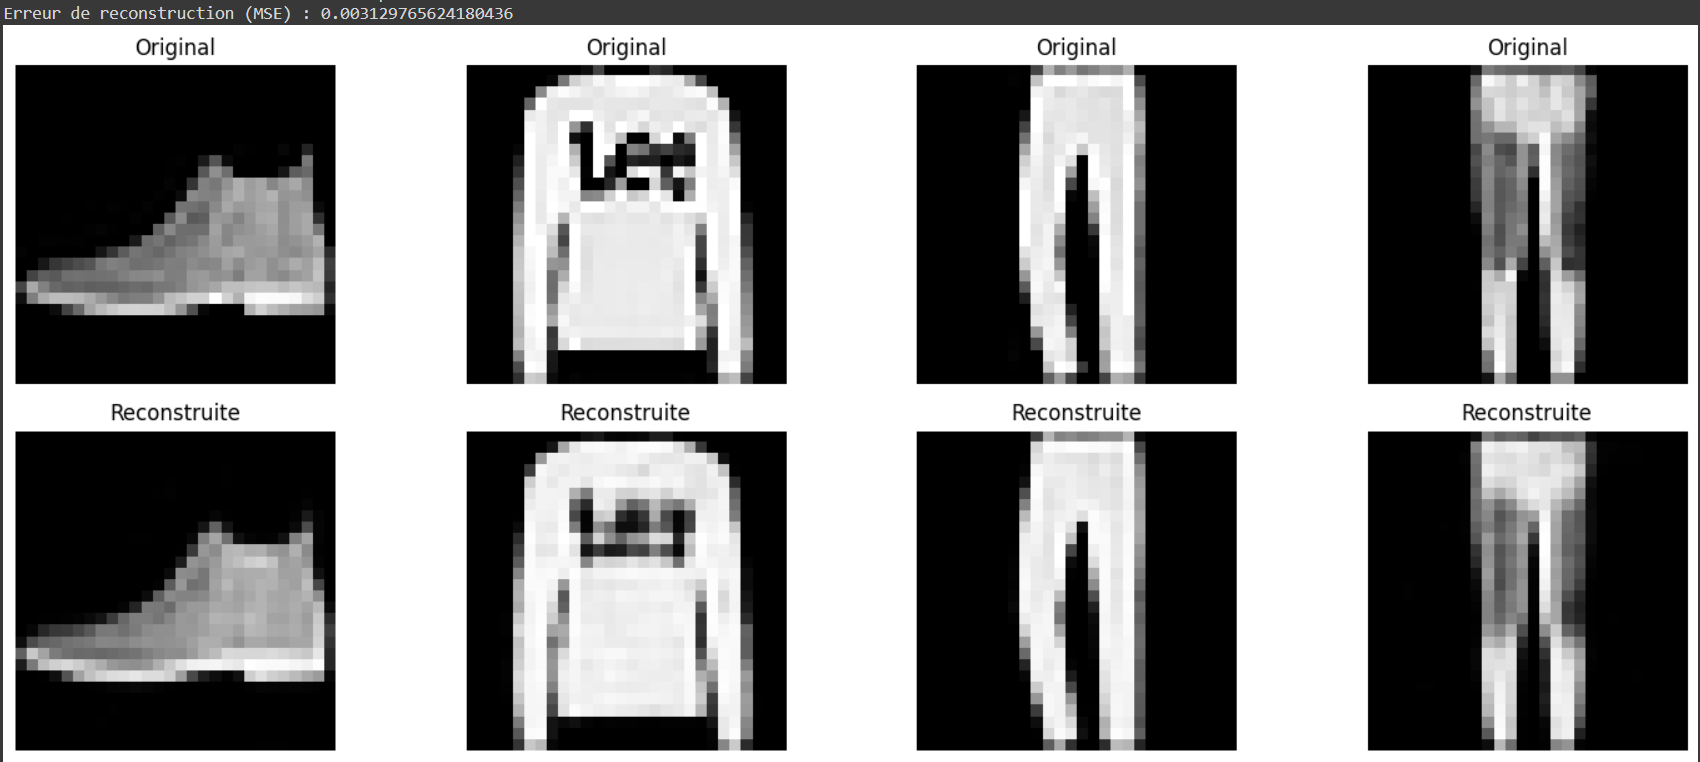
\includegraphics[width=\columnwidth]{Fig/reconstruction_test_autoencoders.png}
        \caption{Exemples de reconstruction des images sur le set de test par l'autoencodeur}
        \label{fig:reconstruction_test}
    \end{figure}

    \item \textbf{Conservation de l'Information} : La visualisation t-SNE en 2d des représentations latentes et des représentations d'origine a révélé une séparation meilleure des différentes catégories de vêtements dans la représentation réduite, indiquant que l'information discriminante était bien préservée et bien captée dans l'espace réduit, en particulier pour la classe "pantalon" qui semble avoir des caractéristiques uniques.
    \begin{figure}[H]
        \centering
        \begin{minipage}[b]{0.45\columnwidth}
            \centering
            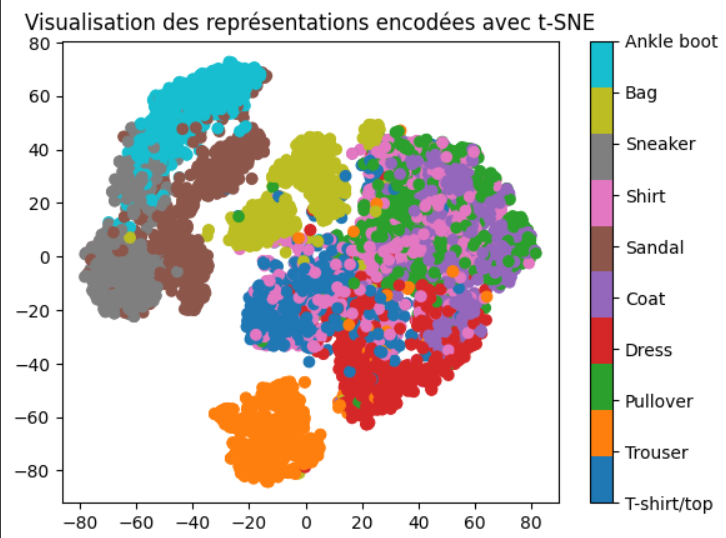
\includegraphics[width=\columnwidth]{Fig/tsnee_latent.png}
            \caption{t-SNE des représentations latentes}
            \label{fig:tsnee_latent}
        \end{minipage}
        \hspace{0.05\columnwidth}
        \begin{minipage}[b]{0.45\columnwidth}
            \centering
            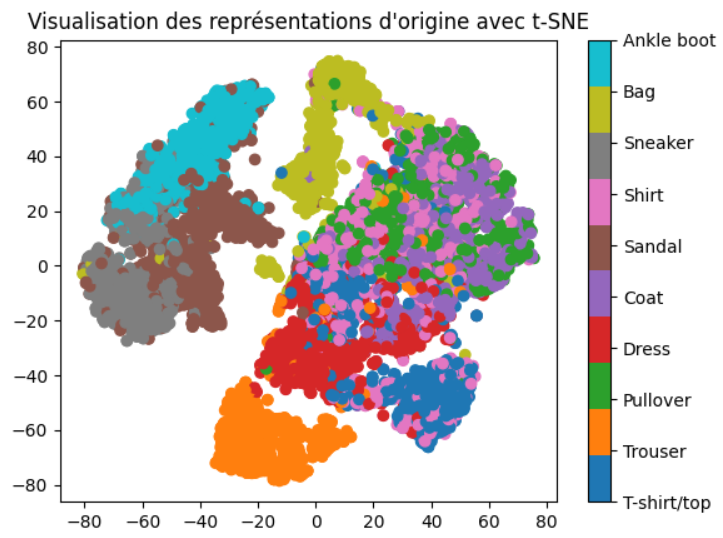
\includegraphics[width=\columnwidth]{Fig/tsnee_origine.png}
            \caption{t-SNE des données originales}
            \label{fig:tsnee_origine}
        \end{minipage}
    \end{figure}
    
    \item \textbf{Comparaison avec PCA} : Les projections PCA des données originales et encodées confirment que l'Auto-Encodeur a capturé dans un espace de l'ordre de 10 fois moindre, l'essentiel de l'information de séparabilité des classes. la distribution des classes dans les 3 premières composantes principales est plus claire dans l'espace réduit.
    \begin{figure}[H]
        \centering
        \begin{minipage}[b]{0.45\columnwidth}
            \centering
            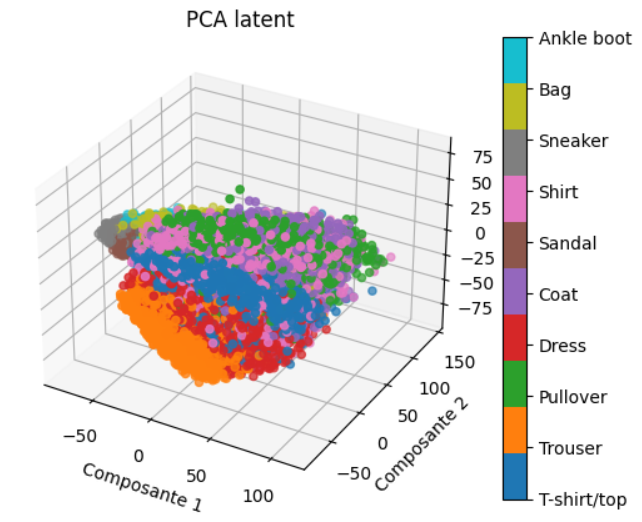
\includegraphics[width=\columnwidth]{Fig/pca_latent.png}
            \caption{PCA des représentations latentes}
            \label{fig:pca_latent}
        \end{minipage}
        \hspace{0.05\columnwidth}
        \begin{minipage}[b]{0.45\columnwidth}
            \centering
            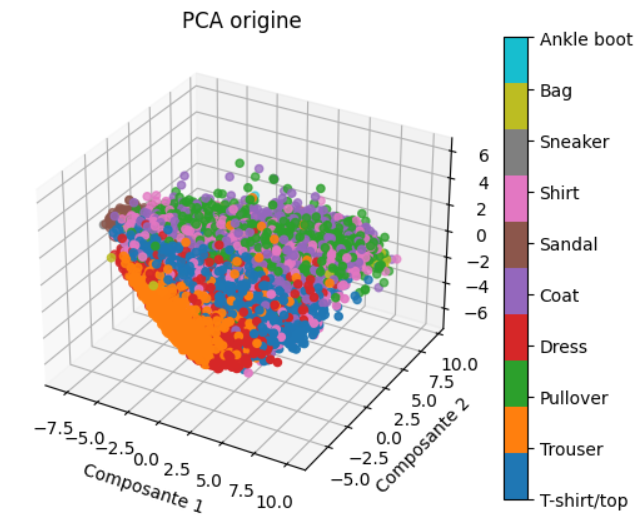
\includegraphics[width=\columnwidth]{Fig/pca_origine.png}
            \caption{PCA des données originales}
            \label{fig:pca_origine}
        \end{minipage}
    \end{figure}
\end{itemize}


\paragraph{Évaluation de la Qualité de la Réduction}
Pour évaluer la pertinence de l'information conservée, nous avons comparé les performances d'un classifieur (régression logistique) sur les données originales et sur les représentations latentes. Les résultats pour un nombre maximal d'itérations de 500 sont résumés dans le tableau ci-dessous :

\begin{table}[h]
\centering
\begin{tabular}{|c|c|c|}
\hline
\textbf{Métrique} & \textbf{Origine} & \textbf{Latent} \\ \hline
Accuracy          & 84.38\%           & 85.00\%         \\ \hline
Precision         & 84.25\%           & 84.84\%         \\ \hline
Recall            & 84.38\%           & 85.00\%         \\ \hline
F1-Score          & 84.29\%           & 84.89\%         \\ \hline
\end{tabular}
\caption{Comparaison des performances de la régression logistique sur l'espace d'origine et l'espace latent, max_iter=500}
\end{table}

Ces résultats montrent que l'Auto-Encodeur a réussi à préserver, voire améliorer légèrement, l'information essentielle pour la classification, malgré une réduction significative de la dimensionnalité. La précision sur l'espace latent (85.00\%) dépasse légèrement celle sur l'espace d'origine (84.38\%), suggérant que la compression réalisée par l'Auto-Encodeur permet une représentation plus efficace de l'information pertinente pour la tâche de classification.
Il est raisonnable d'affirmer que l'Auto-Encodeur a permis une compression sans perte significative de qualité pour la classification, et qu'il a amélioré légèrement la qualité de la prédiction, probablement grâce à l'élimination du bruit à la classification , c'est à dire les caractéristiques non descriminantes des classes.




\section{Discussion}

Notre étude comparative a mis en lumière les forces et les faiblesses de chaque méthode de réduction de dimensionnalité :

\begin{itemize}
    \item \textbf{PCA} s'est révélée efficace pour les structures linéaires et robuste au bruit, mais limitée pour capturer des relations non linéaires complexes.
    \item \textbf{ISOMAP} a excellé dans la préservation de la structure globale des manifolds non linéaires, mais a montré des limitations pour les données très bruitées ou les structures très complexes.
    \item \textbf{LLE} a démontré une forte capacité à préserver les relations locales, mais s'est avérée sensible au bruit et moins performante pour les structures globales complexes.
    \item Les \textbf{Auto-Encoders} ont montré une grande adaptabilité et des performances solides sur une variété de structures de données, mais au prix d'un temps de calcul plus élevé et d'une complexité accrue dans le réglage des hyperparamètres.
\end{itemize}

Ces résultats corroborent largement les conclusions de la littérature existante \cite{vandermaaten2009dimensionality, wang2021comprehensive}. Ils soulignent l'importance de choisir la méthode de réduction de dimensionnalité en fonction de la nature spécifique des données et des objectifs de l'analyse.

L'expérience sur Fashion-MNIST a particulièrement mis en évidence la capacité des Auto-Encoders à préserver l'information discriminante dans un contexte de classification d'images, suggérant leur pertinence pour les tâches de vision par ordinateur.

\section{Conclusion}
Cette étude comparative offre un aperçu pratique des performances de quatre méthodes de réduction de dimensionnalité largement utilisées. Nos résultats soulignent qu'il n'existe pas de méthode universellement supérieure, mais que le choix dépend fortement de la structure des données et des objectifs spécifiques de l'analyse.

Les perspectives futures incluent l'exploration de méthodes plus récentes comme t-SNE ou UMAP, ainsi que l'investigation de l'impact de la réduction de dimensionnalité sur d'autres tâches d'apprentissage automatique au-delà de la classification.

Cette étude, dans un cadre de consolidation des connaissances en fin du module Manifold learning, a clairement contribué à une meilleure compréhension des forces et des limites des différentes approches de réduction de la dimensionnalité expérimentées.

\bibliographystyle{unsrt}
\bibliography{references}
\begin{appendices}

\appendixpage

\section{Visualisations 2D des espaces réduits des données simulées}


\thispagestyle{empty}
\vspace*{\fill}  % Ajoute de l'espace en haut de la page
\begin{figure}[b]  % Utilise [b] pour forcer l'image en bas de la page
    \centering
    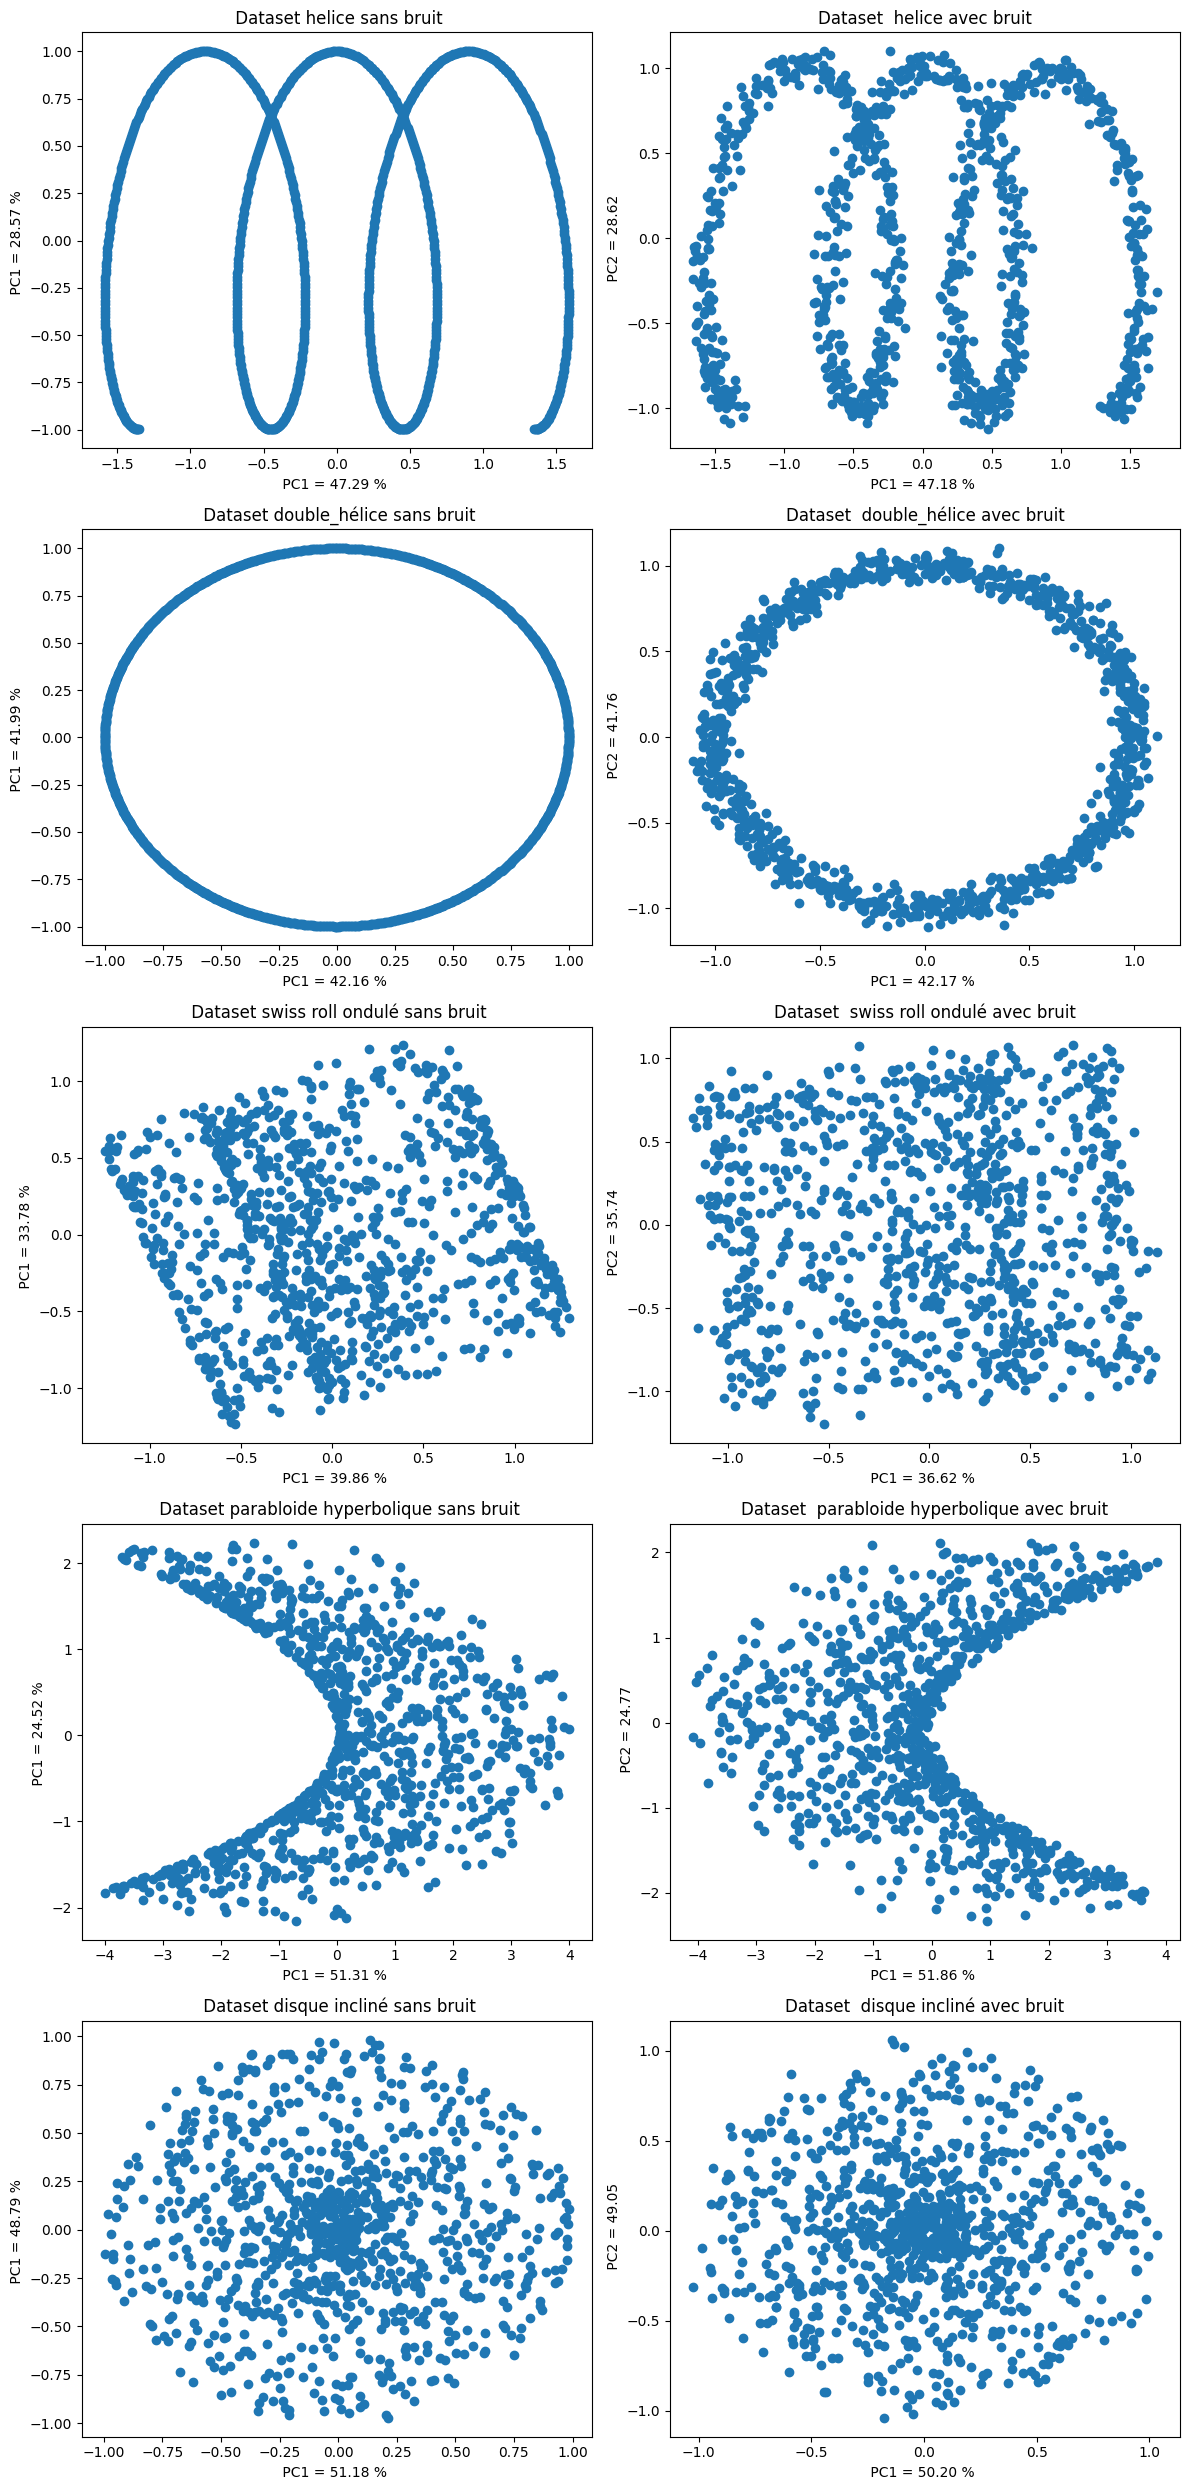
\includegraphics[width=\textwidth,height=0.8\textheight,keepaspectratio]{PCA.png}
    \caption{Résultats de la méthode PCA sur les ensembles de données synthétiques avec et sans bruit.}
    \label{fig:resultats_PCA}
\end{figure}
\vspace*{\fill}  % Ajoute de l'espace en bas de la page

\newpage
\thispagestyle{empty}
\vspace*{\fill}  % Ajoute de l'espace en haut de la page
\begin{figure}[b]
    \centering
    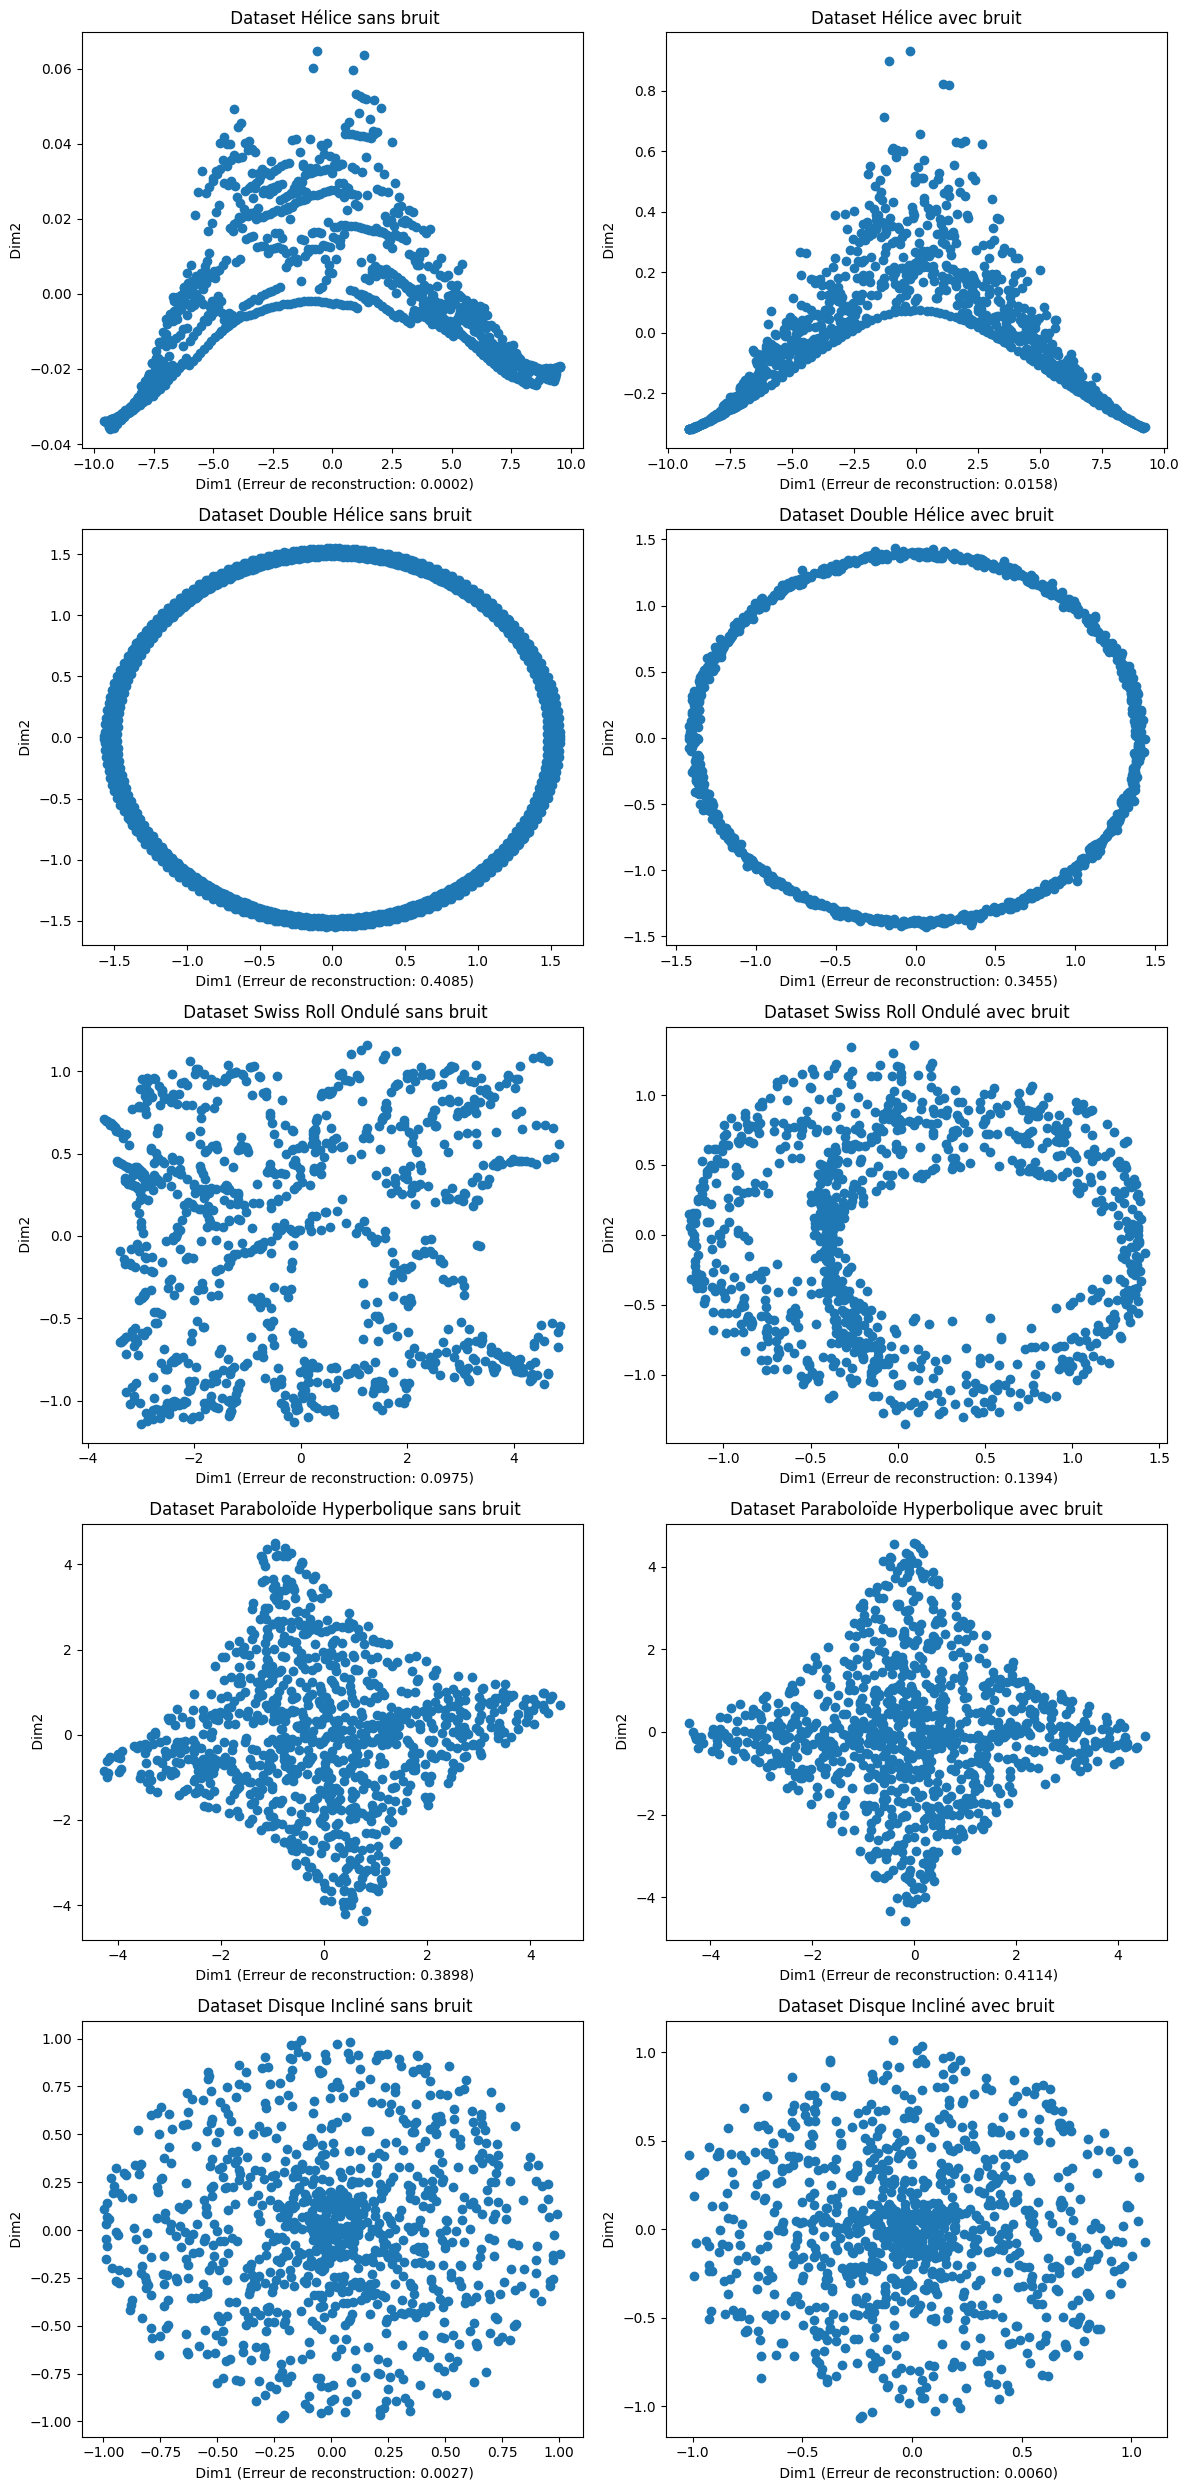
\includegraphics[width=\textwidth,height=0.8\textheight,keepaspectratio]{ISOMAP.png}
    \caption{Résultats de la méthode ISOMAP sur les ensembles de données synthétiques avec et sans bruit.}
    \label{fig:resultats_ISOMAP}
\end{figure}
\vspace*{\fill}

\newpage
\thispagestyle{empty}
\vspace*{\fill}
\begin{figure}[b]
    \centering
    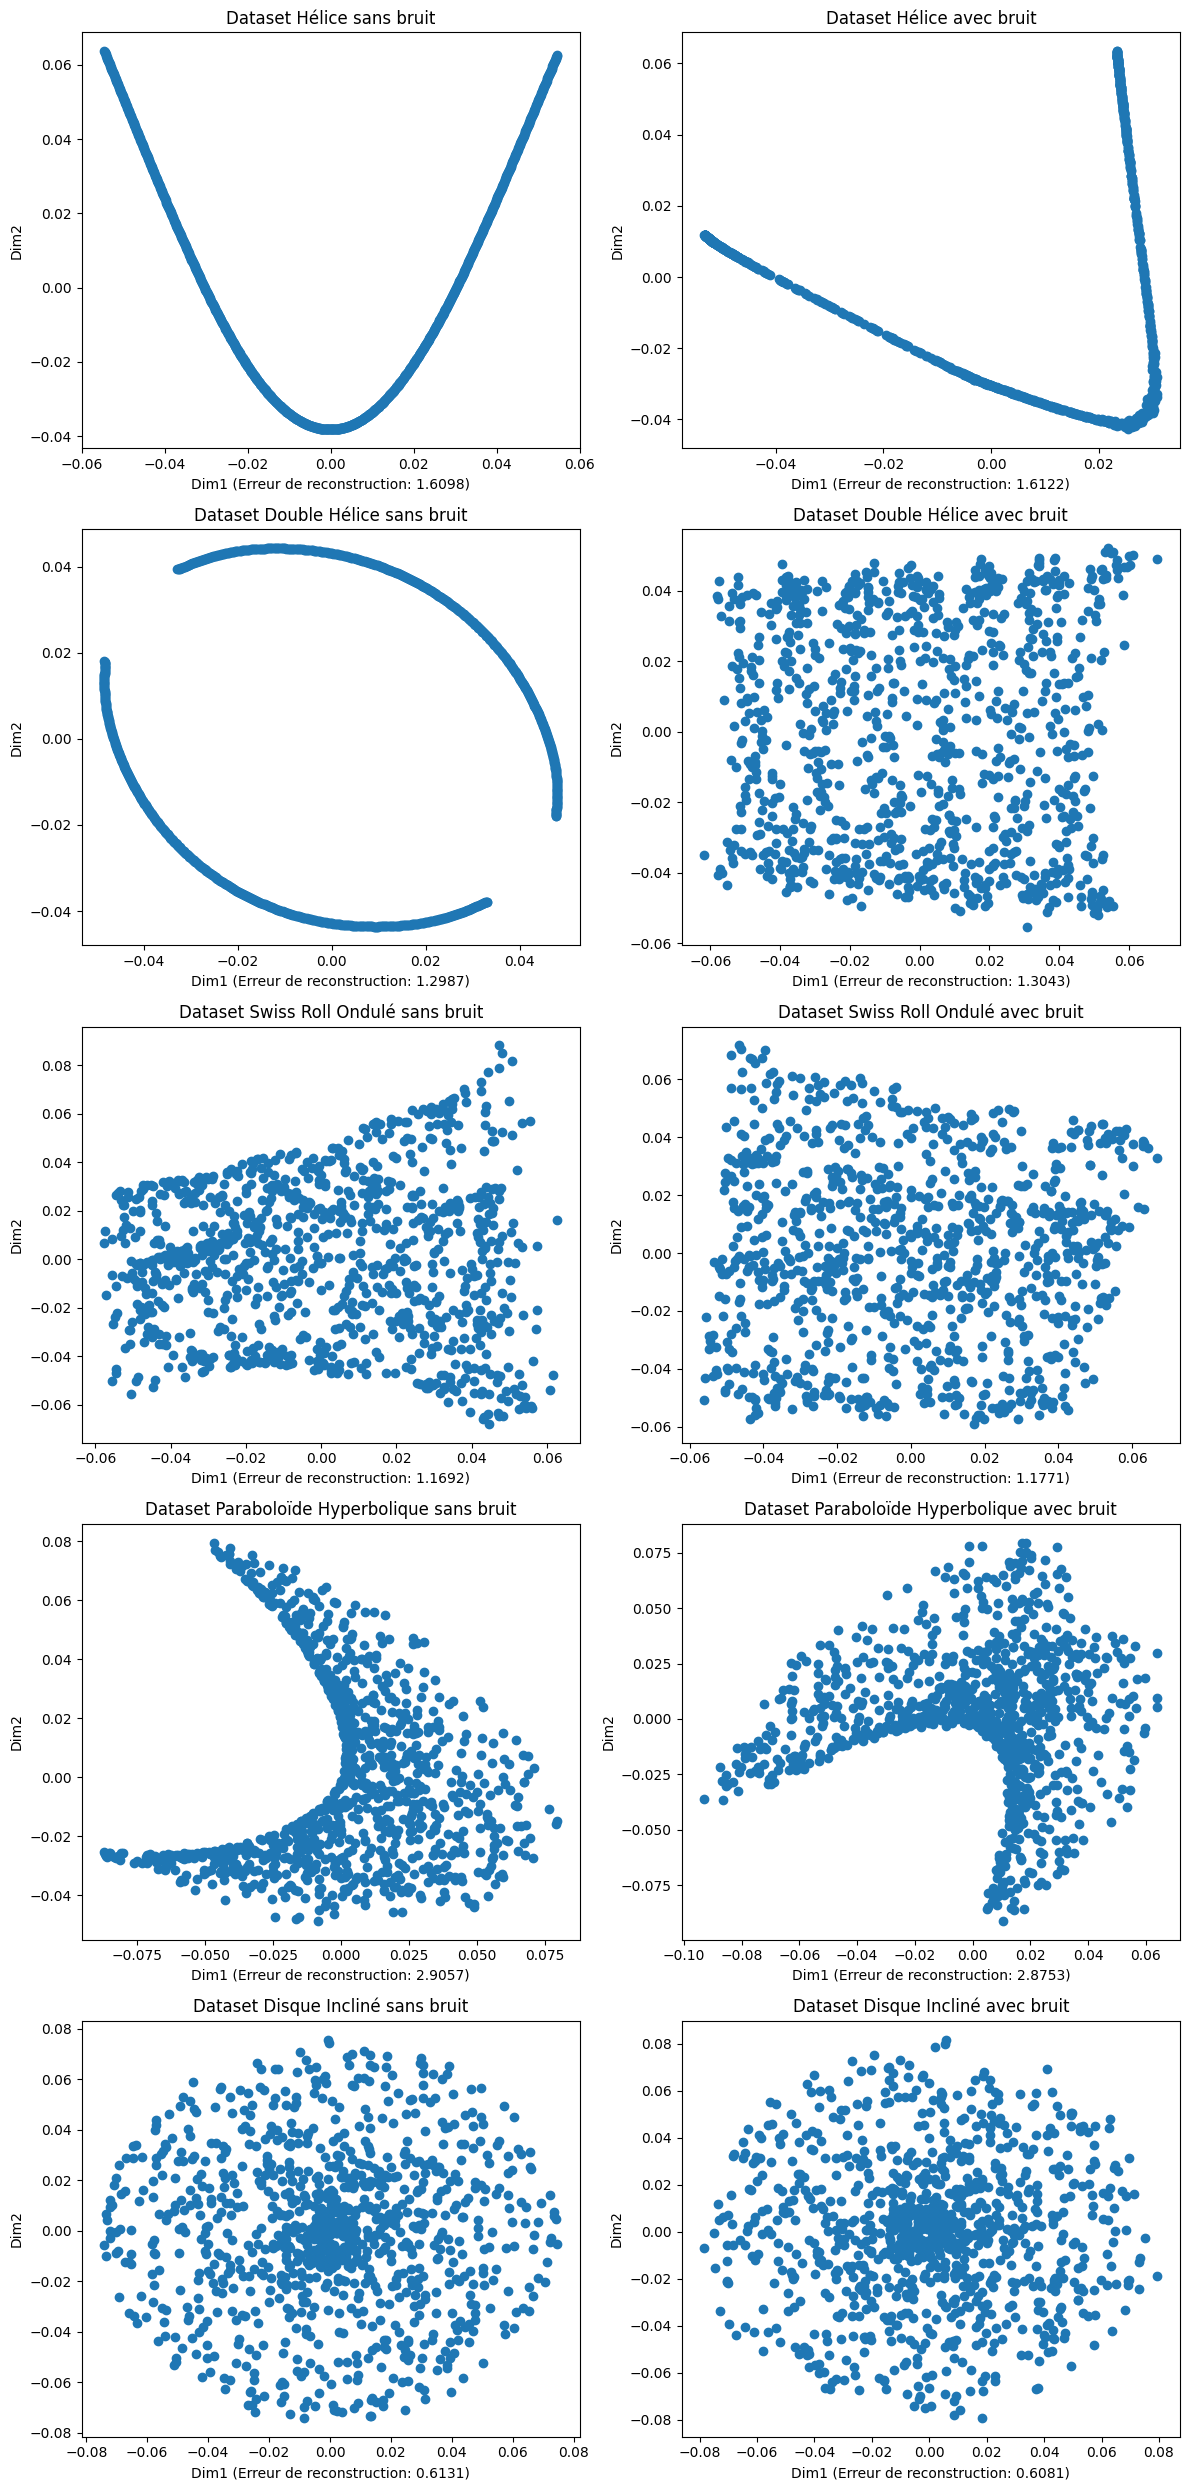
\includegraphics[width=\textwidth,height=0.8\textheight,keepaspectratio]{LLE.png}
    \caption{Résultats de la méthode LLE sur les ensembles de données synthétiques avec et sans bruit.}
    \label{fig:resultats_LLE}
\end{figure}
\vspace*{\fill}

\newpage
\thispagestyle{empty}
\vspace*{\fill}
\begin{figure}[b]
    \centering
    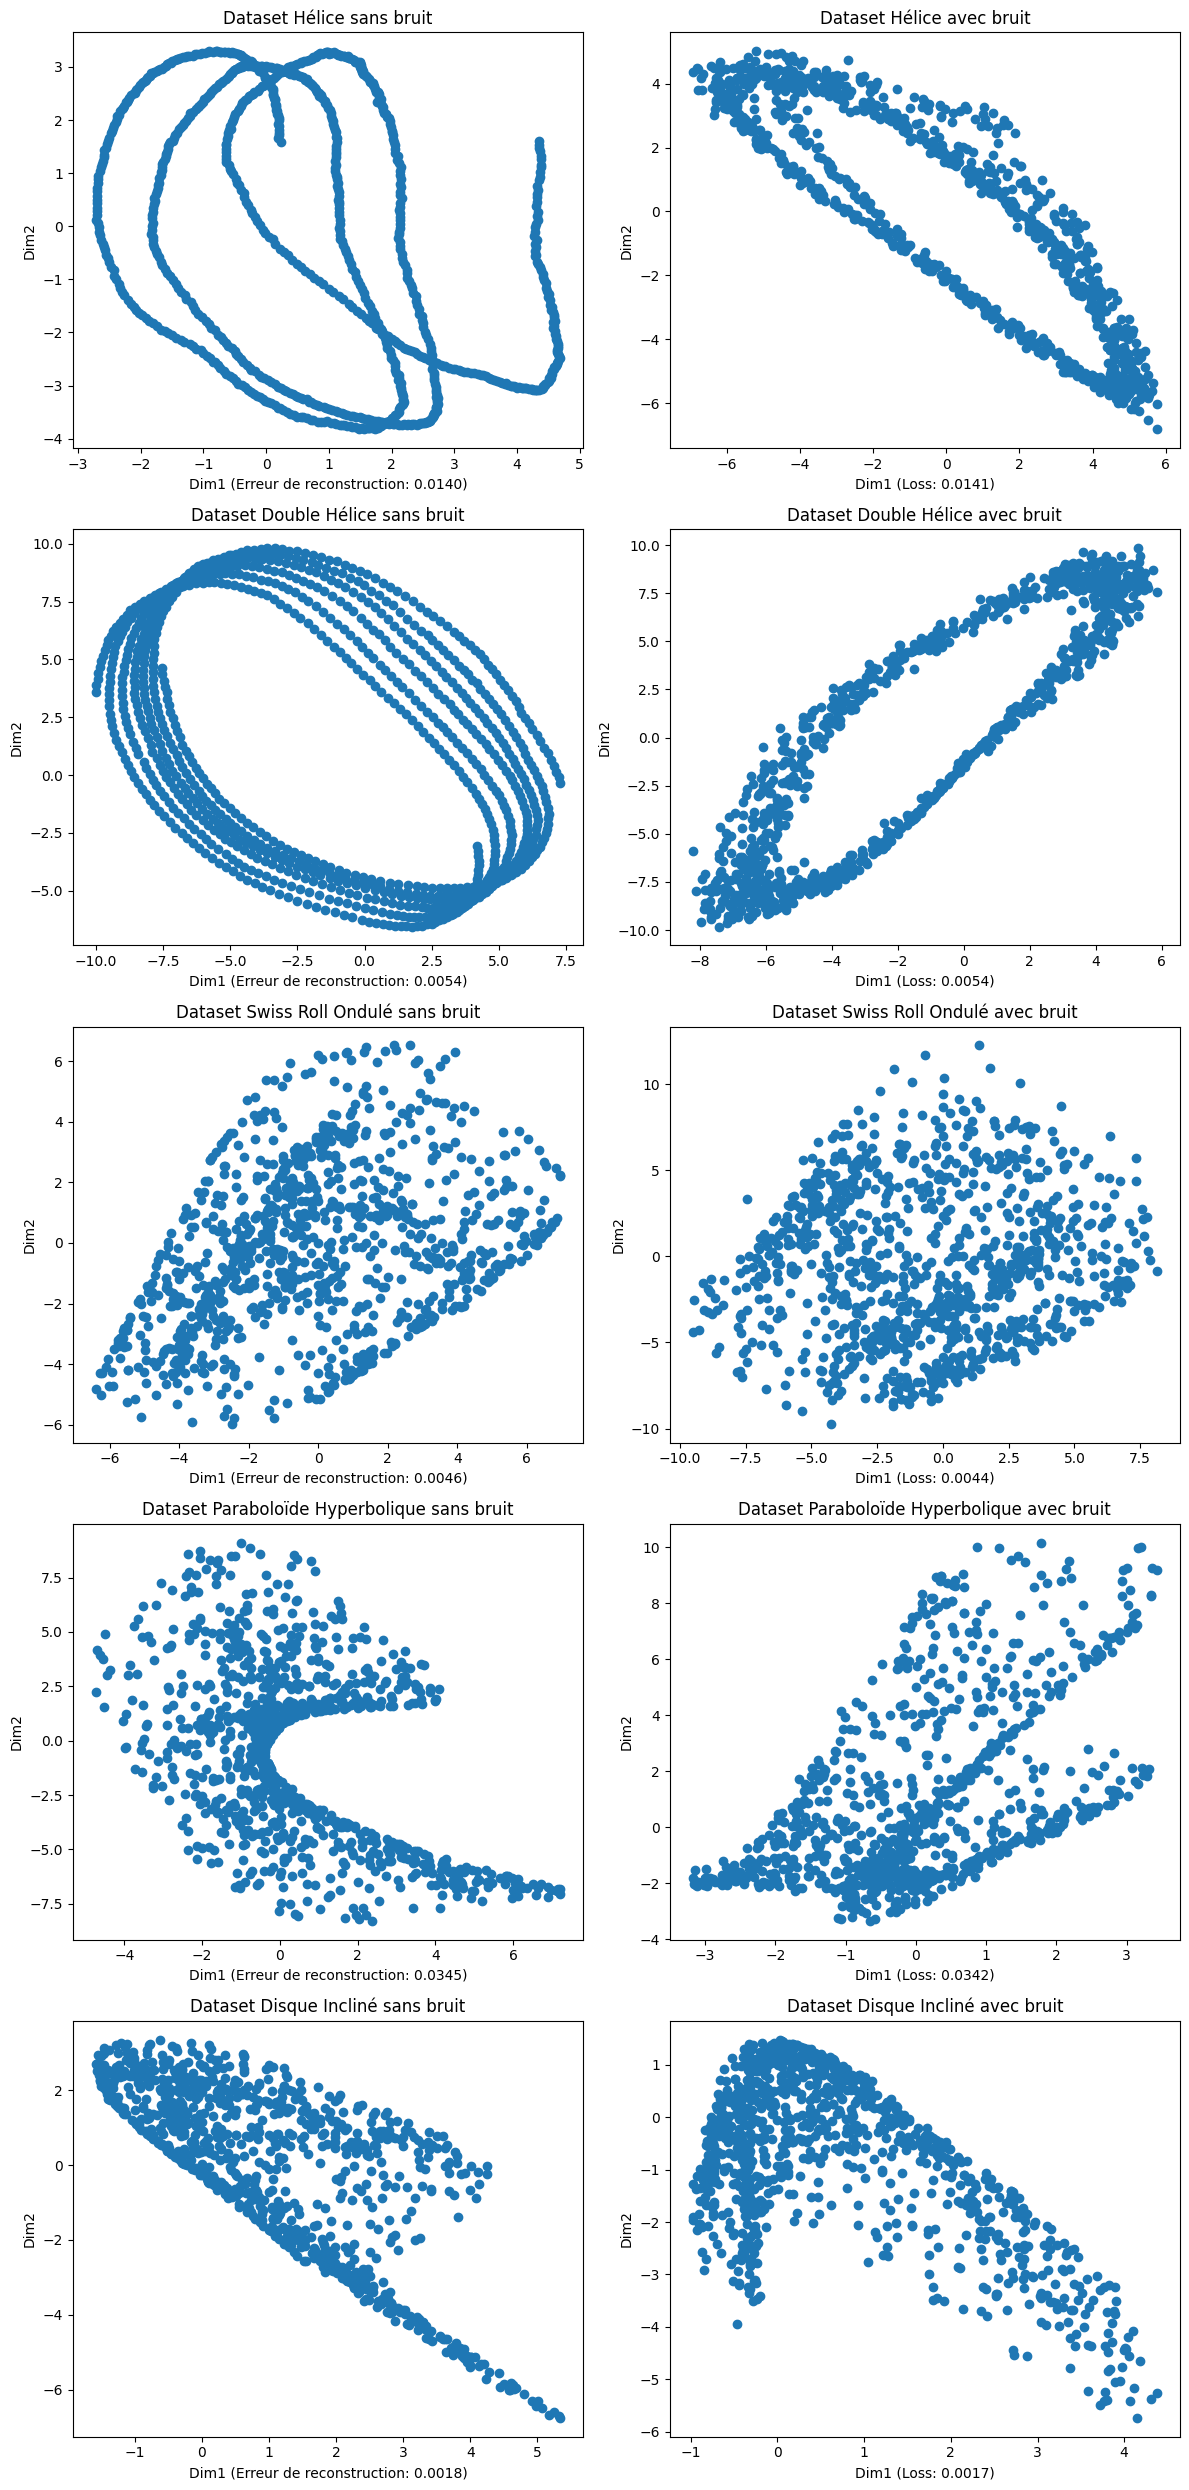
\includegraphics[width=\textwidth,height=0.8\textheight,keepaspectratio]{AE.png}
    \caption{Résultats de la méthode Auto-Encoders sur les ensembles de données synthétiques avec et sans bruit.}
    \label{fig:resultats_AE}
\end{figure}
\vspace*{\fill}

\end{appendices}





\end{document}




\section{Acknowledgments}
The authors thank the anonymous reviewers for their valuable suggestions. This work is supported in part by funds from the National Science Foundation (NSF: \# 1636933 and \# 1920920).


